\documentclass[
  bibliography=totoc,     % Literatur im Inhaltsverzeichnis
  captions=tableheading,  % Tabellenüberschriften
  titlepage=firstiscover, % Titelseite ist Deckblatt (Finnd ich nicht so gut)
]{scrartcl}

% Paket float verbessern
\usepackage{scrhack}

% Warnung, falls nochmal kompiliert werden muss
\usepackage[aux]{rerunfilecheck}

% unverzichtbare Mathe-Befehle
\usepackage{amsmath}
% viele Mathe-Symbole
\usepackage{amssymb}
% Erweiterungen für amsmath
\usepackage{mathtools}

%\usepackage{physics}

% Fonteinstellungen
\usepackage{fontspec}
% Latin Modern Fonts werden automatisch geladen
% Alternativ zum Beispiel:
%\setromanfont{Libertinus Serif}
%\setsansfont{Libertinus Sans}
%\setmonofont{Libertinus Mono}

% Wenn man andere Schriftarten gesetzt hat,
% sollte man das Seiten-Layout neu berechnen lassen
\recalctypearea{}

% deutsche Spracheinstellungen
\usepackage[ngerman]{babel}


\usepackage[
  math-style=ISO,    % ┐
  bold-style=ISO,    % │
  sans-style=italic, % │ ISO-Standard folgen
  nabla=upright,     % │
  partial=upright,   % ┘
  warnings-off={           % ┐
    mathtools-colon,       % │ unnötige Warnungen ausschalten
    mathtools-overbracket, % │
  },                       % ┘
]{unicode-math}

% traditionelle Fonts für Mathematik
\setmathfont{Latin Modern Math}
% Alternativ zum Beispiel:
%\setmathfont{Libertinus Math}

\setmathfont{XITS Math}[range={scr, bfscr}]
\setmathfont{XITS Math}[range={cal, bfcal}, StylisticSet=1]

% Zahlen und Einheiten
\usepackage[
  locale=DE,                   % deutsche Einstellungen
  separate-uncertainty=true,   % immer Unsicherheit mit \pm
  per-mode=symbol-or-fraction, % / in inline math, fraction in display math
]{siunitx}

% chemische Formeln
\usepackage[
  version=4,
  math-greek=default, % ┐ mit unicode-math zusammenarbeiten
  text-greek=default, % ┘
]{mhchem}

% richtige Anführungszeichen
\usepackage[autostyle]{csquotes}

% schöne Brüche im Text
\usepackage{xfrac}

% Standardplatzierung für Floats einstellen
\usepackage{float}
\floatplacement{figure}{htbp}
\floatplacement{table}{htbp}

% Floats innerhalb einer Section halten
\usepackage[
  section, % Floats innerhalb der Section halten
  below,   % unterhalb der Section aber auf der selben Seite ist ok
]{placeins}

% Seite drehen für breite Tabellen: landscape Umgebung
\usepackage{pdflscape}

% Captions schöner machen.
\usepackage[
  labelfont=bf,        % Tabelle x: Abbildung y: ist jetzt fett
  font=small,          % Schrift etwas kleiner als Dokument
  width=0.9\textwidth, % maximale Breite einer Caption schmaler
]{caption}
% subfigure, subtable, subref
\usepackage{subcaption}

% Grafiken können eingebunden werden
\usepackage{graphicx}
\usepackage{wrapfig}

% schöne Tabellen
\usepackage{booktabs}

% Verbesserungen am Schriftbild
\usepackage{microtype}

% Literaturverzeichnis
\usepackage[
  backend=biber,
  sorting=none
]{biblatex}
% Quellendatenbank
\addbibresource{lit.bib}
\addbibresource{programme.bib}

% Hyperlinks im Dokument
\usepackage[
  german,
  unicode,        % Unicode in PDF-Attributen erlauben
  pdfusetitle,    % Titel, Autoren und Datum als PDF-Attribute
  pdfcreator={},  % ┐ PDF-Attribute säubern
  pdfproducer={}, % ┘
]{hyperref}
% erweiterte Bookmarks im PDF
\usepackage{bookmark}

% Trennung von Wörtern mit Strichen
\usepackage[shortcuts]{extdash}

%\setcounter{tocdepth}{3} % + subsubsections



\author{%
  Clara Sondermann \\%
  \href{mailto:clara.sondermann@tu-dortmund.de}{clara.sondermann@tu-dortmund.de}%
  \and%
  Enno Wellmann \\%
  \href{mailto:enno.wellmann@tu-dortmund.de}{enno.wellmann@tu-dortmund.de}%
}
\publishers{TU Dortmund – Fakultät Physik}


\newcommand*\diff{\mathop{}\!\mathrm{d}}

\NewDocumentCommand \OverfullCenter {+m} {
\noindent\makebox[\linewidth]{#1} }

\usepackage{adjustbox}


\title{Versuch 207: Kugelfall-Viskosimeter nach Höppler}
\date{Durchführung: 22.11.2022, Abgabe: 29.11.22}


\begin{document}
\maketitle

\tableofcontents
\newpage



\section{Ziel}
In diesem Versuch wird die dynamische Viskosität\footnote{Nicht zu verwechseln mit der \textit{kinematischen} Viskosität.
Im folgenden wird die \textit{dynamische} Viskosität mit Viskosität bezeichnet.} $\eta$ 
von destilliertem Wasser in Abhängigkeit der Temperatur mit Hilfe des Kugelfall-Viskosimeters nach Höppler ermittelt.



\section{Grundlagen}
\label{sec:grundlagen}
Reale Stoffe (d.h. Flüssigkeiten oder Gase) sind \textit{strömend}, wenn sie einen makroskopischen Impuls haben.
Die thermische Bewegung der einzelnen Moleküle kann dabei vernachlässigt werden.
Die Strömung kann mit Hilfe der Strömungsgeschwindigkeit $\symbf{u}\left(\symbf{r},t\right)$ beschrieben werden.
Als \textit{Stromlinie} oder \textit{Stromfaden} bezeichnet man die Ortskurve, die ein Flüssigkeitselement, etwa ein Korkstück, durchläuft.
Eine Stromlinie wird durch Reibungskräfte im Medium beeinflusst \cite[]{demtroeder}.
Ein Maß für die Stärke der inneren Reibung bzw. die Zähigkeit des Stoffes ist die \textit{dynamische Viskosität} $\eta$ mit der SI-Einheit $\unit{\Pa \s}$.
Diese ist eine temperaturabhängige Materialkonstante \cite[]{geschke}.
Man unterscheidet hierbei zwischen idealen bzw. nicht-viskosen Stoffen, für die $\eta \simeq 0$ gilt, und viskosen Stoffen,
deren Strömungsverhalten in laminar und turbulent eingeteilt wird (vgl. Abschnitt \ref{sec:vorbereitung}).

Die Reibung, die eine Kugel mit Radius $r$ und Geschwindigkeit $v$ in einem Fluid erfährt wird mit Hilfe der Stokesschen Reibung 

\begin{align}
    F_R = 6 \pi \eta v r    
\end{align}

beschrieben.
Sie wirkt mit der Auftriebskraft $\symbf{F}_A$ der Schwerkraft $\symbf{F}_g$ entgegen. 
Mit steigender Geschwindigkeit $v$ wächst die Reibungskraft $\symbf{F}_R$, bis sich ein Kräftegleichgewicht einstellt
und $v$ einen konstanten Wert annimmt.
Dabei wird die Viskosität des Fluids mit der empirischen Formel 

\begin{align}
    \label{eq:empirisch}
    \eta = K \left(\rho_K -\rho_{Fl}\right) \cdot t
\end{align}

ermittelt, wobei $K$ eine Apparaturkonstante ist, die Fallhöhe und Kugelgeometrie berücksichtigt,
$\rho_K$ bzw. $\rho_{Fl}$ die Dichte der Kugel bzw. des Fluids sind und $t$ die Fallzeit darstellt.


Durch die \textit{Andradesche Gleichung} wird die Temperaturabhängigkeit der Viskosität von Flüssigkeiten dargestellt.
\begin{equation}
\label{eq:andrade}
    \eta \left(T\right) = A \exp{\left(\frac{B}{T}\right)}
\end{equation}
$A$ und $B$ sind dabei Konstanten \cite*[]{va207}.





\section{Vorbereitungsaufgaben}
\subsection{Laminare Strömung und Reynoldszahl}
\label{sec:vorbereitung}
Von einer laminaren Strömung wird gesprochen, wenn in einem realen Stoff
die einzelnen Stromfäden ohne sich zu beeinflussen nebeneinander liegen. Das bedeutet, dass es keine Wirbel oder
Turbulenzen innerhalb des Stoffes gibt und sich die einzelnen Schichten mit Strömungsgeschwindigkeiten nicht vermischen.
Die \textit{Reynoldszahl} $Re$ ist ein Maß dafür, ob es sich um eine laminare oder turbulente Strömung handelt.
\noindent
\begin{align}
    Re = \frac{\rho \overline{v} R}{\eta}
    \label{eq:reynold}
\end{align}
Dabei ist $\rho$ die Dichte des Fluids, $\overline{v}$ die relative mittlere Geschwindigkeit zwischen Fluid und Körper und
$R$ die charakteristische Länge.
Wenn die Reynoldszahl unterhalb einer kritischen Grenze $Re_c$ liegt, kann von einer laminaren Strömung gesprochen werden.
Die charakteristische Länge $R$ ist hier der Durchmesser der Kugel und die kritische Grenze der Reynoldszahl $Re_c$ beträgt ca. 2300 \cite*[]{geschke}.


\subsection{Temperaturabhängige Viskosität und Dichte von destilliertem Wasser}
Die Dichte $\rho$ von Wasser hat ihren Maximalwert bei $T_{max} = \qty[]{4}{\degreeCelsius}$ \cite*[]{geschke}.
Außerdem ist $\rho$ im festen Aggregatszustand geringer als im flüssigen Zustand. 
Diese beiden Tatsachen werden auch als \enquote{Dichteanomalie des Wassers} bezeichnet\cite*[]{demtroeder}.
Die Viskosität $\rho$ fällt exponentiell mit dem Kehrwert der Temperatur $\frac{1}{T}$ (vgl. \eqref{eq:andrade}).



\input{durchführung.tex}

%%%%%%%%%%%%%%%%%%%%%%%%%%%%% Section Messdaten entfernen und in der Auswertung einfügen.

\section{Messdaten}
%\subsection{Kenngrößen der Kugeln}

Anfangs wurden die relevanten Kenngrößen der Kugeln bestimmt.
Die Massen sind vorgegeben.
Die Zimmertemperatur betrug stets $T_{Zt}=\qty[]{19}{\degreeCelsius}$.

%%%%%%%%\begin{table}[]
%%%%%%%%    \caption[]{Kenngrößen der kleinen und der großen Kugel. Masse $m$, Durchmesser $d$ und Dichte $\rho$.}
%%%%%%%%    \label{tab:kenngroessen}
%%%%%%%%    \centering
%%%%%%%%    \begin{tabular}[]{S S[table-format=1.4] S[table-format=2.2] @{${}\pm{}$} S[table-format=0.2]}
%%%%%%%%        \toprule
%%%%%%%%        {Kugel} & {$m / \unit{\g}$} & \multicolumn{2}{c}{$d / \unit{\mm}$}   \\
%%%%%%%%        \midrule
%%%%%%%%        {klein} & 4.4531 & 15.61 & 0.01 \\
%%%%%%%%        {groß}  & 2.9528 & 15.78 & 0.01 \\
%%%%%%%%        \bottomrule 
%%%%%%%%
%%%%%%%%    \end{tabular}
%%%%%%%%\end{table}
%ich fand das so als Tabelle etwas schöner hihi :D
%ich weiß nur nicht warum ziwschen Durchmesser und Fehler so eine Lücke ist...
%Lösung: Die Überschrift war zu breit. Mit nur d/mm passt es besser


%\subsection{Messreihe 1: kleine Kugel, konstante Temperatur}

\begin{table}[]
    \caption{Kleine Kugel bei Zimmertemperatur; Fallhöhe = 10 cm}
    \label{tab:klKu_Zitemp}
    \centering
    \sisetup{table-format=2.2}
    \begin{tabular}{S S}
        \toprule
        \multicolumn{2}{c}{Fallzeit $ t / \unit{\s}$}\\
        {oben} & {unten}\\
        \midrule
        12.21 &  12.66 \\
        12.40 &  12.00 \\
        12.25 &  12.32 \\
        12.65 &  12.06 \\
        12.16 &  12.32 \\
        12.13 &  12.09 \\
        12.50 &  12.15 \\
        12.38 &  12.18 \\
        12.34 &  12.38 \\
        12.22 &  12.32 \\
        \bottomrule

    \end{tabular}
\end{table}



\begin{table}[]
    \caption{Große Kugel bei Zimmertemperatur; Fallhöhe = 5 cm}
    \label{tab:grKu_Zitemp}
    \centering
    \sisetup{table-format=2.2}
    \begin{tabular}{S S}
        \toprule
        \multicolumn{2}{c}{Fallzeit $ t / \unit{\s}$}\\
        {oben} & {unten}\\
        \midrule
            34.78 &  34.75 \\
            34.65 &  34.94 \\
            35.00 &  36.90 \\
            35.22 &  35.63 \\
            35.47 &  35.78 \\
        \bottomrule

    \end{tabular}
\end{table}

%\subsection{Messreihe 3: große Kugel, steigende Temperatur}


\begin{table}[]
    \caption{Große Kugel bei variabler Temperatur T; Fallhöhe = 5 cm}
    \label{tab:grKu_steigendeTemp}
    \centering
    \sisetup{table-format=2.2}
    \begin{tabular}{S[table-format=2.0] S S S[table-format=2.0] S S}
        \toprule
        & \multicolumn{2}{c}{Fallzeit $ t / \unit{\s}$} & & \multicolumn{2}{c}{Fallzeit $ t / \unit{\s}$} \\
        {T / \unit{\celsius}} & {oben} & {unten} & {T / \unit{\celsius}} & {oben} & {unten}\\
        \midrule
            26 & 31.37 &  31.22 &  38 & 24.69 &  24.81 \\
               & 30.66 &  31.19 &     & 24.93 &  24.97 \\
            27 & 30.43 &  31.12 &  40 & 23.81 &  23.78 \\
               & 30.37 &  30.63 &     & 23.31 &  23.09 \\
            30 & 29.03 &  29.78 &  43 & 22.28 &  22.37 \\
               & 28.82 &  28.53 &     & 22.35 &  22.15 \\
            32 & 27.63 &  27.96 &  48 & 20.57 &  21.00 \\
               & 28.10 &  28.10 &     & 20.32 &  20.78 \\
            35 & 25.82 &  25.81 &  52 & 19.65 &  19.09 \\
               & 25.68 &  26.16 &     & 19.46 &  19.16 \\   
        \bottomrule
    \end{tabular}
\end{table}


\section{Auswertung}
%\subsection{Fehlerrechnung}

\subsubsection{Gaußsche Fehlerfortpflanzung}

Wenn zu Messdaten die Standardabweichung bekannt ist, und mit diesen Messdaten weiter gerechnet werden soll,
wird die Gaußsche Fehlerfortpflanzung verwendet. 
Angenommen wir haben $k$ Messwerte $x_i [i \in \mathbb{N}, i \leq k]$ mit den Standardabweichungen $\Delta x_i$
und eine abgeleitete Größe $f(x_i)$ dann ist der Fehler von $f$
\begin{align}
    \Delta f(x_i) = \sqrt{
    \left(\frac{\partial f}{\partial x_1} \Delta x_1\right)^2%
     + \left(\frac{\partial f}{\partial x_2} \Delta x_2\right)^2%
     + \dots%
     + \left(\frac{\partial f}{\partial x_k} \Delta x_k\right)^2%
    }.
    \label{eq:gauspflanz}
\end{align} 
Im Ergebnis gibt es dann den Mittelwert von $f$ mit der errechneten Abweichung $\overline{f} \pm \Delta f $.
Um Rechenfehler zu vermeiden wird das Python Paket \texttt{uncertainties} \cite[][]{uncertainties} verwendet.
Hier wird die Fehlerfortpflanzung automatisch verrechnet, wenn man die Variablen als \texttt{ufloat} definiert.


%\subsubsection{Fehlerrechnung bei der linearen Regression}
%%% Die Inhalte zur Fehlerrechnung werden dahin kopiert wo sie als erstes verwendet werden.

\subsection{Kenngrößen der Glaskugeln}


Wie bereits in Abschnitt \ref{sec:durchfuehrung} erwähnt, werden die Massen $m$ der Kugeln vorgegeben
und die Durchmesser $d$ mit der Schieblehre bestimmt.
Die Werte sind in Tabelle \ref{tab:Dichten} angegeben.
Wenn zu Messdaten die Standardabweichung bekannt ist, und mit diesen Messdaten weiter gerechnet werden soll,
wird die Gaußsche Fehlerfortpflanzung verwendet. 
Angenommen es gibt $k$ Messwerte $x_i ~[i \in \mathbb{N}, i \leq k]$ mit den Standardabweichungen $\Delta x_i$
und eine abgeleitete Größe $f(x_i)$, dann ist der Fehler von $f$
\begin{align}
    \Delta f(x_i) = \sqrt{
    \left(\frac{\partial f}{\partial x_1} \Delta x_1\right)^2%
     + \left(\frac{\partial f}{\partial x_2} \Delta x_2\right)^2%
     + \dots%
     + \left(\frac{\partial f}{\partial x_k} \Delta x_k\right)^2%
    }.
    \label{eq:gauspflanz}
\end{align} 
Im Ergebnis gibt es dann den Mittelwert von $f$ mit der errechneten Abweichung $\overline{f} \pm \Delta f $.
%Um Rechenfehler zu vermeiden wird das Python Paket \texttt{uncertainties} \cite[][]{uncertainties} verwendet.
%Hier wird die Fehlerfortpflanzung automatisch verrechnet, wenn man die Variablen als \texttt{ufloat} definiert.
%Die Gaußsche Fehlerfortpflanzung \eqref{eq:gauspflanz} wird hier das erste Mal verwendet.
Die Standard-Messunsicherheit der Schieblehre wird mit $\qty{0.01}{\mm}$ angegeben.
Die Dichte $\rho$ errechnet sich aus dem Verhältnis zwischen Masse $m$ und Volumen.
\begin{align*}
    V &= \frac{4 \pi}{3} \left(\frac{d}{2}\right)^3 & \rho &= \frac{m}{V} &
    \frac{\partial \rho}{\partial d} &= -\frac{18 m}{\pi} d^{-4} %
\end{align*}
%%%%%
%\rho &= \frac{m}{V} = \frac{3 m}{4 \pi} \left(  \frac{2}{d} \right)^{3} = \frac{6 m}{\pi} d^{-3} \\%
%
Da für die Masse keine Standardabweichung gegeben ist, enthält die Gaußsche Fehlerfortpflanzung nur einen Summanden unter der Wurzel.
\begin{align*}
    \Delta \rho &= \sqrt{\left(\frac{\partial \rho}{\partial d} \right)^{2} \Delta d^{2} }%
    =\sqrt{\left(-\frac{18 m}{\pi} d^{-4} \right)^{2} \Delta d^{2} }%
\end{align*}%
Für die Dichten $\rho$ der Kugeln folgen somit die Werte in Tabelle \ref{tab:Dichten}.



\begin{table}
    \caption{Die Dichten $\rho$}
    \label{tab:Dichten}
    \centering
    \begin{tabular}[]{S S[table-format=1.4] S[table-format=2.2] @{${}\pm{}$} S[table-format=0.2] S[table-format=1.4] @{${}\pm{}$} S[table-format=0.2]}
        \toprule
        {Kugel} & {$m / \unit{\g}$} & \multicolumn{2}{c}{$d / \unit{\mm}$}  & \multicolumn{2}{c}{{$\rho / \left( \unit{\g \per \cubic\cm}\right)$}} \\
        \midrule
        {klein} & 4.4531 & 15.61 & 0.01 & 2.2359 & 0.005\\
        {groß}  & 2.9528 & 15.78 & 0.01 & 2.4073 & 0.005\\
        %                        \pm             \pm
        \bottomrule 

    \end{tabular}
\end{table}
%Um Rechenfehler zu vermeiden werden für die konkrete Berechnung der Messunsicherheiten 
%das Python-Paket uncertainties \cite{uncertainties} \cite{python} verwendet.




\subsection{Messreihe 1: kleine Kugel, konstante Temperatur}
\label{sec:auswertung_mr1}
%
\subsubsection[]{Arithmetisches Mittel und Standardabweichung}
Bei Messungen von denen die Standardmessunsicherheit nicht bekannt ist, 
ist es sinnvoll mehrere Messungen zu machen und von ihnen das arithmetische Mittel zu bilden.
So entsteht eine genauere Messung. % Überdenken
Das arithmetische Mittel einer Messreihe mit $N$ Werten $x_i$ wird folgendermaßen berechnet:
\begin{align}
    \overline{x} = \frac{1}{N} \sum_{i=1}^{N}x_i
    \label{eq:artim_mit}
\end{align}
%
Der Standardmessfehler des arithmetischen Mittels der Messreihe berechnet sich dann wie folgt:
\begin{align}
    \Delta \overline{x} = \sqrt[]{\frac{1}{N \left(N-1\right)} \sum_{k=1}^{N} \left(x_{i} - \overline{x}\right)^2}
    \label{eq:stddev_mit}
\end{align}
%
%
\subsubsection[]{Fallzeiten der kleinen Kugel}
In der ersten Messreihe werden die Fallzeiten für die kleinere Kugel gemessen.
Das Wasser hat eine Zimmertemperatur von \qty{19}{\celsius} 
und die Fallstrecke beträgt \qty[]{10}{\cm}. 
Somit ergeben sich die Daten in Tabelle \ref{tab:klKu_Zitemp}.
\begin{table}%[h!]
    \caption{Fallzeiten der kleinen Kugel bei Zimmertemperatur}
    \label{tab:klKu_Zitemp}
    \centering
    \sisetup{table-format=2.2}
    \begin{tabular}{S S}
        \toprule
        \multicolumn{2}{c}{Fallzeit $ t_\text{klein} / \unit{\s}$}\\
        {oben} & {unten}\\
        \midrule
        12.21 &  12.66 \\
        12.40 &  12.00 \\
        12.25 &  12.32 \\
        12.65 &  12.06 \\
        12.16 &  12.32 \\
        12.13 &  12.09 \\
        12.50 &  12.15 \\
        12.38 &  12.18 \\
        12.34 &  12.38 \\
        12.22 &  12.32 \\
        \bottomrule
    \end{tabular}
\end{table}
%
Das arithmetischen Mittel der Laufzeiten $\overline{t_\text{oben}}$ und $\overline{t_\text{unten}}$
werden nach \eqref{eq:artim_mit} für $N= 10$ Werte aus Tabelle \ref{tab:klKu_Zitemp} berechnet.
Die Standardmessfehler des Mittelwertes werden gemäß \eqref{eq:artim_mit} berechnet.
Die Ergebnisse sind in Tabelle \ref{tab:mittel_fallzeit_klein} einzusehen.
%
\begin{table}[H]
    \centering
    \caption{Durchschnittliche Fallzeiten für die kleine Kugel}
    \label{tab:mittel_fallzeit_klein}
    \sisetup{table-format=2.2}
    \begin{tabular}[]{c S @{${}\pm{}$} S}
        \toprule
        Ausrichtung   & \multicolumn{2}{c}{$\overline{t_\text{klein}} / \unit{\s}  $} \\
        \midrule
        oben  & \num{12.32} &  \num{0.16}    \\
        unten & \num{12.25} &  \num{0.18}    \\
        \bottomrule
        \end{tabular}
\end{table}
%
%
% Alte Version:
%%%%%Für die kleine Kugel oben ergibt sich mit Tabelle \ref{tab:klKu_Zitemp} 
%%%%%also für die Fallzeit ein arithmetisches Mittel von%
%%%%%%
%%%%%\begin{align*}
%%%%%    \overline{t_{\text{kl, oben}}} &= \frac{1}{10} \sum_{k=1}^{10} {t_{\text{kl, oben}, k}} = \qty[]{12.324}{\s}\\%
%%%%%%
%%%%%\intertext{mit einer Standardabweichung von}%
%%%%%%
%%%%%    \Delta \overline{t_{\text{kl, oben}}} &= 
%%%%%    \sqrt[]{\frac{1}{90} \sum_{k=1}^{10} \left(t_{\text{kl, oben}, k} - \overline{t}_{\text{kl, oben}}\right)^2}
%%%%%    = \qty[]{0.155}{\s}\\%
%%%%%    %
%%%%%\end{align*}
%%%%%Analog folgt für unten eine Fallzeit von der Mittelwert $\overline{t}_{\text{kl, unten}} = \qty[]{12.248}{\s}$
%%%%%und die Standardabweichung $\Delta\overline{t}_{\text{kl, unten}} = \qty[]{0.184}{\s}$.
%
%Durchschnittszeiten kleine Kugel:
%oben: 12.32400 mit Fehler:  0.15500
%unten: 12.24800 mit Fehler:  0.18405
%
%Durchschnittszeiten grosse Kugel:
%oben: 35.02400 mit Fehler:  0.29574
%unten: 35.60000 mit Fehler:  0.75913
%
%\newpage
\subsubsection[]{Viskosität des Wassers}
Für die kleine Kugel beträgt nach \cite{va207} die Apparatekonstante $K_{\text{klein}} = \qty[]{0.07640}{\milli\Pa \cubic\cm}$.
Nach \cite[][290]{geschke} beträgt bei $T = \qty{19}{\degreeCelsius}$ die Dichte von Wasser $\rho_\text{Fl} = \qty{0.99841}{\g \per \cm^3}$.
Mit Gleichung \eqref{eq:empirisch} folgen somit für die Viskosität $\overline{\eta_{\text{klein}}}$ des Wassers die Werte in Tabelle \ref{tab:visk_kl_Zitemp},
wobei die Fehler gemäß \eqref{eq:gauspflanz} berechnet wurden. 
%%%% Vielleicht muss das an eine frühere Stelle, ich denke aber nicht
% Da für die beiden unterschiedlichen Ausrichtungen des Viskosimeters kleine Unterschiede zu erwarten sind,
% werden die Ergebnisse in $x_\text{oben}$ und in $x_\text{unten}$ aufgeteilt.
% Dies steht dafür auf welcher Seite (oben oder unten) die Schläuche von der Wärmeinheit des 
% Viskosimeters \textbf{Referenz zu Abbildung einfügen} bei der jeweiligen Messung sind.
%
\begin{table}
    \centering
    \caption{Durchschnittliche Viskositäten des Wassers für die kleine Kugel}
    \label{tab:visk_kl_Zitemp}
    \sisetup{table-format=1.3}
    \begin{tabular}[]{c S @{${}\pm{}$} S}
        \toprule
        Ausrichtung   & \multicolumn{2}{c}{$\overline{\eta_{\text{klein}}} / \unit{\milli\pascal\s}  $} \\
        \midrule
        oben & \num{1.165} &  \num{0.015}    \\
        unten & \num{1.158} &  \num{0.018}    \\
        \bottomrule
        \end{tabular}
\end{table}
%Mit Gleichung \eqref{eq:empirisch} folgt somit für die Viskosität oben $\eta_{\text{kl, oben}} = \left(1.165 \pm 0.015\right) 10^{-3} \, \unit{\pascal \s}$
%und unten 
%$\eta_{\text{kl, unten}} = \left(1.158 \pm 0.018\right) 10^{-3} \, \unit{\pascal \s}$.
%%%%%%%%%%%%%% Eigentlich wäre das hier in einer Tabelle viel schöner.
%eta klein oben:  0.001165+/-0.000015
%eta klein unten:  0.001158+/-0.000018


\input{Auswertung/02_große_Kugel_konst_Temp.tex}


\subsection[]{Messreihe 3: Überprüfung der Andradeschen Gleichung}

\begin{figure}
    \centering
    \includegraphics[width=\textwidth]{build/Messreihe3.pdf}
    \caption{Die Fallzeit nach \ref{tab:grKu_steigendeTemp}.}
    \label{fig:groKu_steigendeTemp}
\end{figure}

In dieser Messreihe wird die Temperatur schrittweise erhöht um die Temperaturabhängigkeit der Viskosität herauszufinden.
Die empirische Gleichung für die Viskosität \ref{eq:empirisch} enthält die Dichte des Wassers, die auch temperaturabhängig ist.
In \ref{tab:viskositaeten_temp} werden die Dichten des Wassers aus \cite[][290]{geschke} übernommen. 
Bei den Temperaturen, die nicht in \cite[][290]{geschke} enthalten sind wird auf die nächste angegebene Temperatur gerundet.
%Idee für die Diskussion hier villeicht noch Vergelichswerte aus dem Geschke hinzufügen.
\begin{table}
    \centering
    \sisetup{table-format=1.2}
    \begin{tabular}[]{S[table-format=2.0] S[table-format=0.5] S @{${}\pm{}$} S[table-format=1.3] S @{${}\pm{}$} S[table-format=1.3]}
        \toprule
        {$T /\unit{\celsius}$} & {$\rho_{\text{Wasser}}$ \cite{geschke}} & \multicolumn{2}{c}{$ \eta / \unit{\milli\Pa\s}$} & \multicolumn{2}{c}{$ \eta / \unit{\milli\Pa\s}$} \\
            26  &  0.99679   & 1.03  & 0.021 &        1.02 & 0.027  \\
            27  &  0.99652   & 1.01  & 0.018 &        1.01 & 0.026  \\
            30  &  0.99565   & 0.96  & 0.017 &        0.95 & 0.026  \\
            32  &  0.99565   & 0.93  & 0.028 &        0.91 & 0.028  \\
            35  &  0.994     & 0.86  & 0.015 &        0.85 & 0.030  \\
            38  &  0.9922    & 0.83  & 0.025 &        0.81 & 0.023  \\
            40  &  0.9922    & 0.79  & 0.016 &        0.77 & 0.020  \\
            43  &  0.9902    & 0.75  & 0.04  &        0.73 & 0.04   \\
            48  &  0.988     & 0.69  & 0.012 &        0.69 & 0.019  \\
            52  &  0.988     & 0.66  & 0.020 &        0.63 & 0.028  \\
        	%                        \pm                   \pm 
    \end{tabular}
    \caption{Die Viskosität in Abhängigkeit der Temperatur nach}
    \label{tab:viskositaeten_temp}
\end{table}
\begin{figure}
    \centering
    \includegraphics[width=\textwidth]{build/plot.pdf}
    \caption{Die errechneten Viskositäten in einer logarithmischen Darstellung mit einem linearen Fit}
    \label{fig:groKu_steigendeTemp_eta_fit}
\end{figure}
%
\noindent
Formt man die Andradesche Gleichung \eqref{eq:andrade} so um, dass auf beiden Seiten der Logarithmus gezogen wird, ergibt sich
\begin{align}
    \ln {\left( \eta \right)} = \frac{B}{T} + \ln{\left( A \right)}.
\end{align}
Die Werte für die Viskosität sollten also nach der theoretischen Erwartung linear mit dem inversen der Temperatur zusammenhängen.
Von den zuvor berechneten Werten \ref{tab:viskositaeten_temp} wird der natürliche logarythmus geplottet.
Die lineare Regression mit der \texttt{polyfit} Einstellung \texttt{deg=1} wird gebildet.
Durch das Prinzip der kleinsten Abstandsquadrate entsteht so eine Funktion der Form
\begin{align*}
    f(x) = mx + b
\end{align*}
Für die Parameter ergeben sich die Werte:
\begin{align*}
    m = 1761.27 & b = -5.85
\end{align*}
Dadurch lassen sich die Konstanten $A$ und $B$ ermitteln.


\subsection[]{Die Reynoldszahl}
Um zu ermitteln, ob es sich um eine laminare Strömung handelt, wird jeweils die dimensionslose Reynoldszahl $Re$ für die kleine und große Kugel bestimmt
(vgl. Abschnitt \ref{sec:vorbereitung}).
Zur Berechnung fehlen noch Mittelwert und Standardabweichung der Fallgeschwindigkeit $\overline{v}$ jeweils für oben und unten
(Dichte von Wasser bei Zimmertemperatur: $\rho = \qty{0.99841}{\g \per \cm^3}$, s.o.).

\begin{table}
    \caption[]{Reynoldszahl $Re$ in Abhängigkeit der Fallgeschwindigkeit $\overline{v}$}
    \label{tab:reynold}
    \centering
    \begin{tabular}[]{S S S[table-format=1.4] @{${}\pm{}$} S[table-format=1.4] S[table-format=4.1] @{${}\pm{}$} S[table-format=3.1]}
        \toprule
        {Kugel} & {Strecke} & \multicolumn{2}{c}{$\overline{v} / \left(\unit{\cm\per\s}\right)$} & \multicolumn{2}{c}{$Re$} \\
        \bottomrule
        {klein} & {oben} & 0.811 & 0.010 & 549 & 14 \\
         & {unten} & 0.816 & 0.012 & 555 & 17 \\
        {groß} & {oben} & 0.1428 & 0.0012 & 96.5 & 1.5 \\
         & {unten} & 0.1404 & 0.0030 & 95.5 & 2.5 \\
    \end{tabular}
\end{table}

% Kugel % Strecke % MW G % S G % MW Rey % S Rey
%Reynold:
%Geschwindigkeit klein oben:  0.811+/-0.010
%Geschwindigkeit klein unten:  0.816+/-0.012
%Geschwindigkeit gross oben:  0.1428+/-0.0012
%Geschwindigkeit gross unten:  0.1404+/-0.0030

%rey klein oben:  549+/-14
%rey klein unten:  555+/-17
%rey gross oben:  96.5+/-1.5
%rey gross unten:  95.5+/-2.5


\subsection[]{Die Reynoldszahl}
Um zu ermitteln, ob es sich um eine laminare Strömung handelt, wird jeweils die dimensionslose Reynoldszahl $Re$ für die kleine und große Kugel bestimmt
(vgl. \eqref{eq:reynold}).
Bei höheren Temperaturen können Verwirbelungen entstehen, die dafür sorgen, dass keine laminare Strömung mehr vorliegt.
Das würde bei der Messreihe in Abschnitt \ref{sec:andra_gl} zu Abweichungen von den erwarteten Ergebnissen führen.
Um das zu vermeiden wird die Reynoldszahl für die höchste Temperatur der Messreihe berechnet.
Die Reynoldszahlen für die kleineren Temperaturen sollten kleiner sein, da die Geschwindigkeiten niedriger und die Viskositäten höher sind.
Zur Berechnung fehlen noch Mittelwert und Standardabweichung der Fallgeschwindigkeit $\overline{v}$ jeweils für oben und unten
Die Dichte von Wasser bei Zimmertemperatur beträgt $\rho_{\qty{19}{\celsius}} = \qty{0.99841}{\g \per \cm^3}$ (vgl. \ref{sec:visk_wasser_zt}),
bei $\qty{52}{\celsius}$ beträgt sie $\rho_{\qty{52}{\celsius}} = \qty{0.988}{\g \per \cm^3}$.
Diese werden mit der Gaußschen Fehlerfortpflanzung \eqref{eq:gauspflanz} verrechnet.
%
\begin{table}
    \caption[]{Reynoldszahl $Re$ in Abhängigkeit der Fallgeschwindigkeit $\overline{v}$}
    \label{tab:reynold}
    \centering
    \sisetup{table-format=1.3}
    \begin{tabular}[]{S S S @{${}\pm{}$} S S[table-format=3.0] @{${}\pm{}$} S[table-format=2.0]}
        \toprule
        {Kugel} & {Strecke} & \multicolumn{2}{c}{$\overline{v} / \left(\unit{\cm\per\s}\right)$} & \multicolumn{2}{c}{$Re$} \\
        \midrule
        {klein} & {oben} & 0.811 & 0.010 & 549 & 14 \\
         & {unten} & 0.816 & 0.012 & 555 & 17 \\
        {groß} & {oben} & 0.143 & 0.001 & 97 & 2 \\
         & {unten} & 0.140 & 0.003 & 96 & 3 \\
        {groß \qty{52}{\celsius}} & {oben} & \multicolumn{2}{S}{0.256} & 304 & 5 \\
         & {unten} & \multicolumn{2}{S}{0.261} & 325 & 9 \\
        \bottomrule
    \end{tabular}
\end{table}
%
Es zeigt sich: Alle Werte für die Reynoldszahl sind unterhalb der kritischen Grenze von 2300.

% Kugel % Strecke % MW G % S G % MW Rey % S Rey
%Reynold:
%Geschwindigkeit klein oben:  0.811+/-0.010
%Geschwindigkeit klein unten:  0.816+/-0.012
%Geschwindigkeit gross oben:  0.1428+/-0.0012
%Geschwindigkeit gross unten:  0.1404+/-0.0030

%rey klein oben:  549+/-14
%rey klein unten:  555+/-17
%rey gross oben:  96.5+/-1.5
%rey gross unten:  95.5+/-2.5


\section{Diskussion}

Die realen Güteziffern sind in etwa um den Faktor 10 kleiner als die 


\printbibliography

\section{Anhang}
\begin{minipage}[t]{0.45\textwidth}
    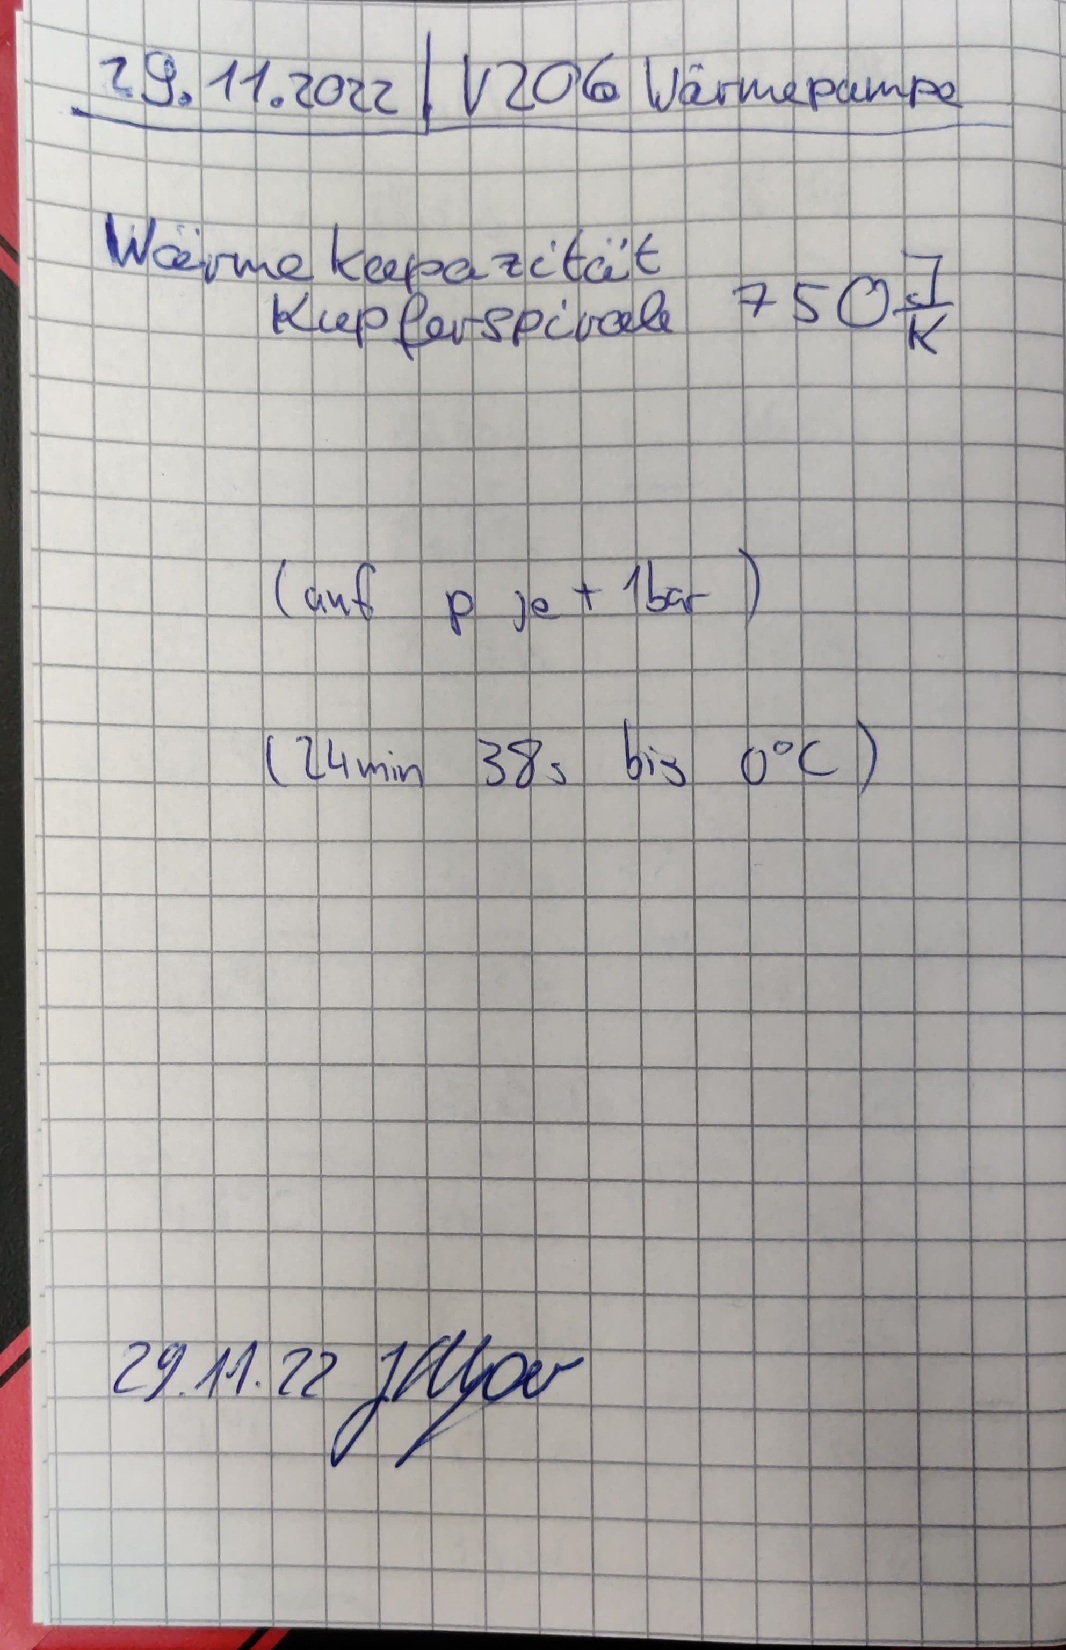
\includegraphics[width=\textwidth, page=1]{v206 Messdaten.pdf}
\end{minipage}
\begin{minipage}[t]{0.45\textwidth}
    \includegraphics[width=\textwidth, keepaspectratio, page=2]{v206 Messdaten.pdf}
\end{minipage}

\begin{minipage}[t]{0.45\textwidth}
    \includegraphics[width=\textwidth, page=3]{v206 Messdaten.pdf}
\end{minipage}

\end{document}